%
% Chapter 11
%

\chapter{RESULTS}
This analysis performs a measurment of the best-fit signal strength, known as $\mu$ of the \tth signal process. This analysis also sets limits
on the SM \tth process. These measurments are the results of 



\begin{table}[htbp]
\begin{center}
  \caption[Table of Final Limits]{95$\%$ CL upper limits on $\mu$ under the background-only hypothesis.}
    \begin{tabular}{c c} \hline
      Observed Limit & Expected Limit $\pm$1$\sigma$  \\ \hline 
      2.9 & 1.0$^{+0.5}_{-0.3}$  \\
      \hline
    \end{tabular}
    \label{tab:limits}
\end{center}
\end{table}

\begin{table}[htbp]
\begin{center}
  \caption[Table of Signal Strength]{}
    \begin{tabular}{c c c} \hline
      Observed signal strength best-fit $\mu$ $\pm$1$\sigma$ & Expected signal strength best-fit $\mu$ $\pm$1$\sigma$ & Observed(expected) significance & \\ \hline 
      1.7$^{+0.6}_{-.05}$ & 1.0$^{}_{}$ & 3.3$\sigma$ (2.1$\sigma$)  \\
      \hline
    \end{tabular}
    \label{tab:mu}
\end{center}
\end{table}

%% \begin{figure}[hbtp]
%%  \begin{center}
%%    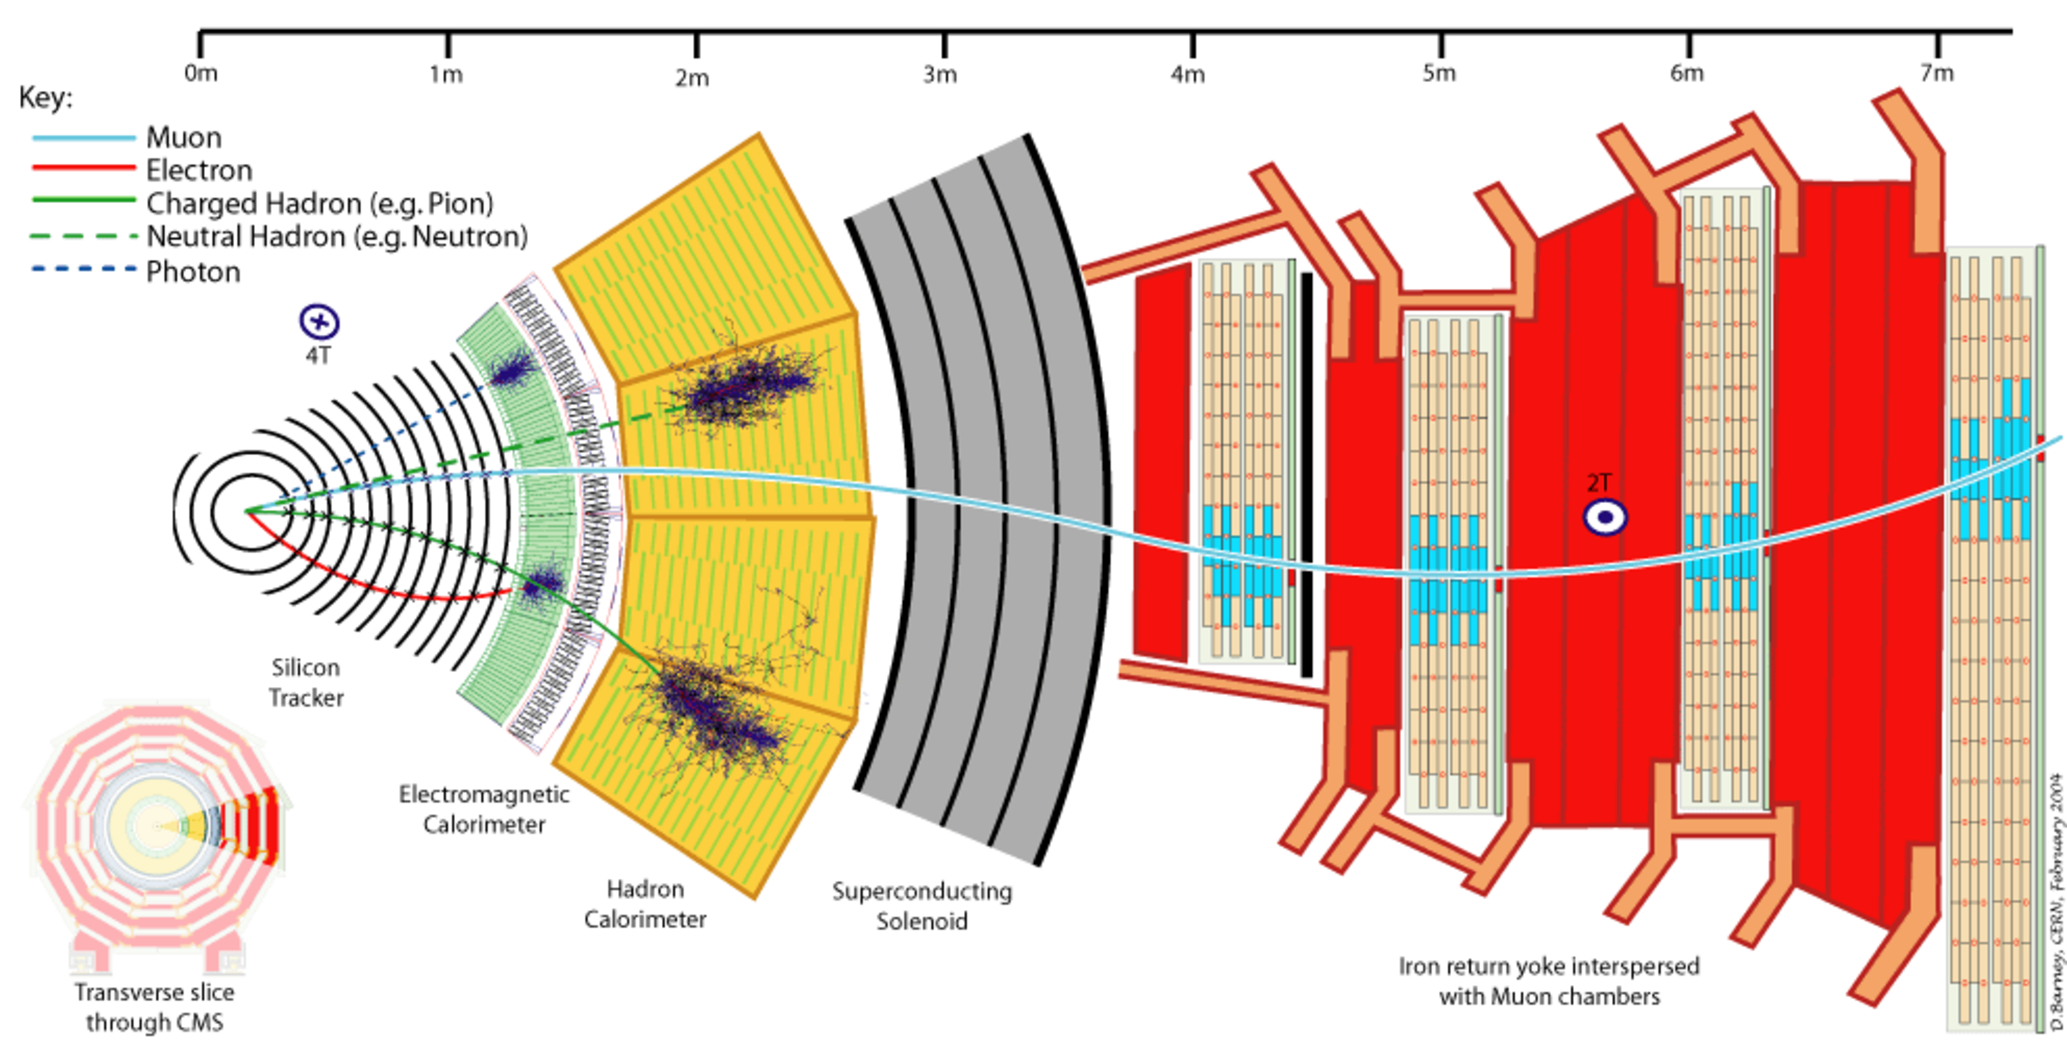
\includegraphics[width=0.8\textwidth]{ch4_figs/cms_particleflow.pdf}
%%    \caption{An overview of how CMS detects different types of particles. The slice of CMS in in the x-y plane.~\cite{NEED CITATION}.}
%%    \label{fig:cms_pflow}
%%  \end{center}
%% \end{figure}
